\newpage
\chapter{Demonstration and Evaluation}
After the system's features have been implemented, the system can be demonstrated and evaluated. This chapter provides a demonstration of the use cases derived from the objective of the thesis, as well as an evaluation of the use cases based on the requirements analysis conducted in \autoref{requirements_analysis}.

\section{Demonstration}
Due to the fact that the extension was originally created for Marta's website, it will be used as an example in the demonstration. The following procedure is illustrated in this chapter as a result of this thesis:

\begin{enumerate}
  \item With the extension installed, visit any webpage with URL path or query
  \item Store the URL path and query in a JSON format
  \item Reload the page
  \item View the number of times URL parameters have been entered by opening the extension's pop-up.
\end{enumerate}

The \texttt{dist} directory is loaded manually to \verb;chrome://extensions; because the extension has not yet been published in the Chrome Web Store. Once the extension has been loaded, it appears in the Chrome Extensions Toolbar. When the extension is opened for the first time, users will be notified that the entries for the specified host are empty (See \autoref{fig:filtreNoEntries}).

\begin{figure}[H]
  \centering
  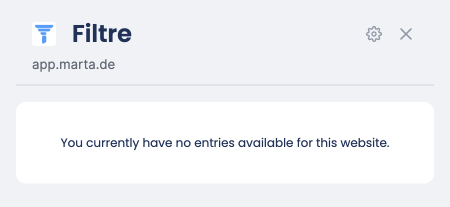
\includegraphics[width=0.7\textwidth]{assets/screenshot_filtre_no_entries.png}
  \caption{Screenshot of the no entries available page}
  \label{fig:filtreNoEntries}
\end{figure}

Families can find suitable caregivers through the Marta webapp at \url{app.marta.de/caregivers}. The page limits search results to 30 caregivers. In addition to the restriction, therefore, a filter based on URL query is implemented, allowing families to filter more caregivers. A modal dialog\footnote{\emph{Modal dialog} is a dialog that appears on top of the primary content and initiates a special mode that requires user interaction. More information on \url{https://www.nngroup.com/articles/modal-nonmodal-dialog/}} is displayed for filter configuration. After modifying the filter settings, the URL becomes \url{app.marta.de/caregivers?caregiver.germanVerbalProficiency=one}. This URL is now stored in the extension's \texttt{chrome.storage}. \autoref{fig:filtreKnownPaths} is a listing of all the top-level paths stored from the website's hostname. Since the user has only visited the \texttt{/caregivers} page, only one item is displayed.

\begin{figure}[H]
  \centering
  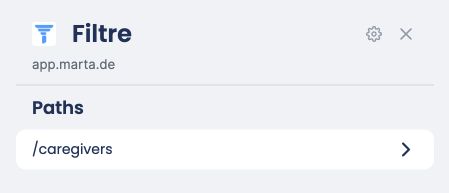
\includegraphics[width=0.7\textwidth]{assets/screenshot_filtre_known_paths.png}
  \caption{Screenshot of the known paths page}
  \label{fig:filtreKnownPaths}
\end{figure}

Clicking on one of the items navigates user to a more refined page inside the extension. \autoref{fig:filtreParameters} displays a list of saved URL subpaths and parameters. The user can see the number of times each parameter is called on the right side of the box, as well as when the parameter was last called below the parameter value, on this page. Reloading the page updates the \texttt{lastUpdatedAt} key and the parameter count

Another thing to note is the input field and the "Navigate" button at the bottom of the page. The value in the input field is updated whenever the user navigates through the extension's "directory path" and selects the parameters. By clicking the "Navigate" button, the user can then navigate to the updated URL in a new tab.

\begin{figure}[H]
  \centering
  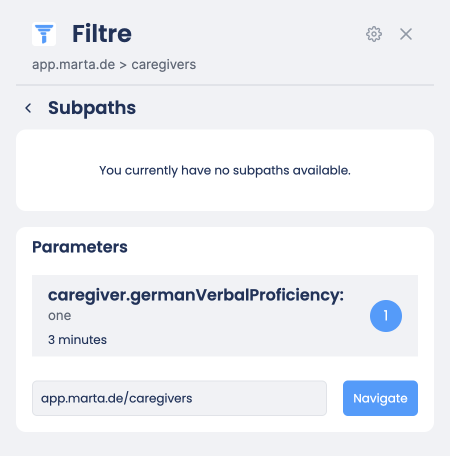
\includegraphics[width=0.7\textwidth]{assets/screenshot_filtre_parameters.png}
  \caption{Screenshot of the known subpaths and parameters page}
  \label{fig:filtreParameters}
\end{figure}

With the help of \emph{Storage Area Explorer}\footnote{\emph{Storage Area Explorer} is a an easy-to-use editor for Chrome Packaged Apps \& Extensions' Storage Area. GitHub repository: \url{https://github.com/jusio/storage-area-explorer}}, it is possible edit or view the \texttt{chrome.storage} using a user interface without the need for console logging the \texttt{chrome.storage} object in the code (See \autoref{fig:storageAreaExplorer}). The current size and size limit are also displayed within the Storage Explorer.

\begin{figure}[H]
  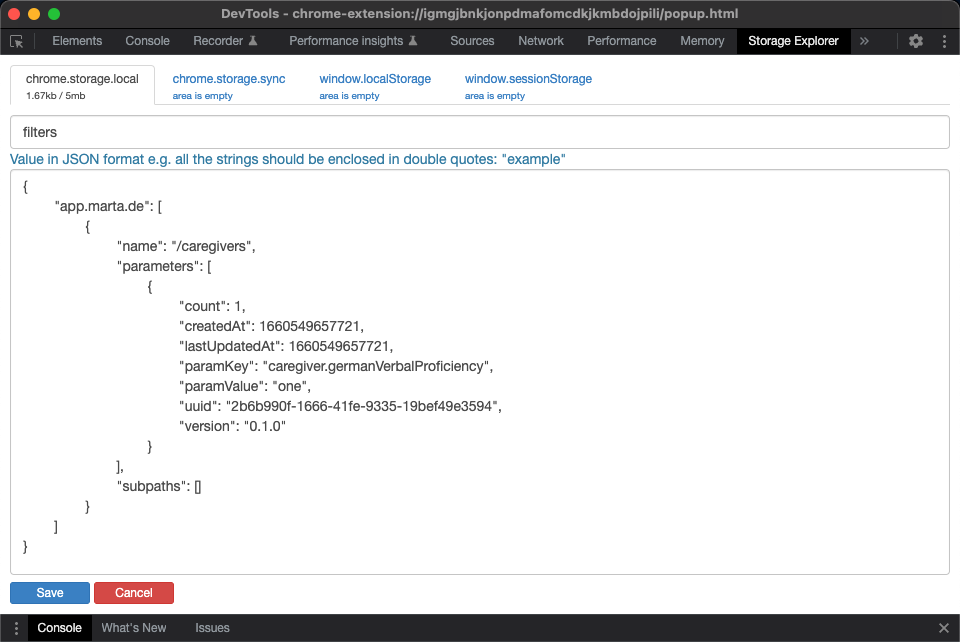
\includegraphics[width=\textwidth]{assets/screenschot_storage_area_explorer.png}
  \caption{Screenshot of the Storage Area Explorer}
  \label{fig:storageAreaExplorer}
\end{figure}

\section{Evaluation}
The achievement of the goals and criteria outlined in the requirement analysis should serve as a metric for determining whether the system and its functionalities have achieved their primary objective in accordance with the thesis objective. \autoref{table:evaluationTableRequirementAnalysis} displays, by requirement identifier, the degree to which the defined requirements have been met:

\begin{tabularx}{\textwidth}{p{0.1\textwidth} p{0.2\textwidth} p{0.6\textwidth}}
  \caption{Evaluation table of requirement analysis}                                                                                                                                                                                                                                                                                                                                                                       \\
  \toprule
  \textbf{ID} & \textbf{Implemented} & \textbf{Remark}                                                                                                                                                                                                                                                                                                                                                                     \\
  \midrule
  FR-01       & \Checkedbox          &                                                                                                                                                                                                                                                                                                                                                                                     \\
  \midrule
  FR-02       & \Checkedbox          & Based on the user's history after installing the extension.                                                                                                                                                                                                                                                                                                                         \\
  \midrule
  FR-03       & \Checkedbox          & It is possible to select multiple parameters. When two identical keys with different values are selected, the second value overwrites the first and no duplicates are produced.                                                                                                                                                                                                     \\
  \midrule
  FR-04       & \Checkedbox          &                                                                                                                                                                                                                                                                                                                                                                                     \\
  \midrule
  FR-05       & \Checkedbox          &                                                                                                                                                                                                                                                                                                                                                                                     \\
  \midrule
  FR-06       & (\Checkedbox)        & The URL is saved but not on each page load because most front-end frameworks nowadays avoid reloading the entire page when navigating through the website. As a result, the URL is now saved whenever the URL value is changed.                                                                                                                                                     \\
  \midrule
  FR-07       & \Checkedbox          &                                                                                                                                                                                                                                                                                                                                                                                     \\
  \midrule
  FR-08       & \HollowBox           & Removing a query parameter count is unnecessary because it contradicts the extension's purpose, which is to suggest the most frequently used filters. The reason this requirement was written in the first place was to allow for customization for a better user experience. Data storage optimization is an option for improvement as data grows and storage capacity is limited. \\
  \midrule
  FR-09       & \Checkedbox          & The Clear All Filter button will prompt the user to type "yes" to ensure that the button is not accidentally clicked. To avoid confusion, the button should be differentiated more.                                                                                                                                                                                                 \\
  \midrule
  FR-10       & \HollowBox           & Reset configuration button is for now not necessary because currently the only available configuration options are "Excluded Parameters".                                                                                                                                                                                                                                           \\
  \midrule
  NFR-01      & \Checkedbox          &                                                                                                                                                                                                                                                                                                                                                                                     \\
  \midrule
  NFR-02      & \Checkedbox          &                                                                                                                                                                                                                                                                                                                                                                                     \\
  \midrule
  NFR-03      & \Checkedbox          &                                                                                                                                                                                                                                                                                                                                                                                     \\
  \midrule
  NFR-04      & \Checkedbox          &                                                                                                                                                                                                                                                                                                                                                                                     \\
  \midrule
  NFR-05      & \Checkedbox          &                                                                                                                                                                                                                                                                                                                                                                                     \\
  \midrule
  NFR-06      & \Checkedbox          &                                                                                                                                                                                                                                                                                                                                                                                     \\
  \midrule
  NFR-07      & \Checkedbox          &                                                                                                                                                                                                                                                                                                                                                                                     \\
  \bottomrule
  \label{table:evaluationTableRequirementAnalysis}
\end{tabularx}

\noindent Minor exceptions notwithstanding, the extension was therefore fully implemented. No usability tests were conducted.

\section{Publish in the Chrome Web Store}
The release of the extension in the Chrome Web Store would allow Google to at least examine the implementation and identify potential vulnerabilities. Nonetheless, the extension must be internationalized beforehand.
